\chapter{Introduction}
\label{ch:Intro}


%%%%%%%%%%%%%%%%%%%%%%%%%%%%%%%%%%%%%%%%%%%%%%%%%%


\section{Psoriasis and psoriatic arthritis}
%
Psoriasis (PSO) and psoriatic arthritis (PsA) are considered different common complex disease entities. PSO is a chronic inflammatory skin disease with episodes of relapse and remitance included in the group of inflammatory dermatose diseases \parencite{Nestle2009}. On the other hand, PsA is a seronegative, chronic, inflammatory disease within the family of spondyloarthritis \parencite{Moll1973, Coates2016}, usually developed after the manifestation of PSO \parencite{Villanova2016}. PS and PsA have both, similar and different, clinical features, which are likely a reflection of shared and individual genetic loci contributing to the disease development (Variants in RUNX3 contribute to susceptibility to PsA, exhibiting further common ground with ankylosing spondylitis, PsA Immunochip). It is important to understand the commonalities and differences between PSO and PsA at the physiological and genetic level in order to better understand the relevance of the genetic variability in the risk to develop these conditions.

\subsection{Epidemiology and global impact}
%
PSO represents a serious global problem that currently affects about 100 million people worldwide, including children and adults regardless sex \parencite{Organization2016}. Although PSO prevalence presents a very weak correlation with geographic latitude \parencite{Jacobson2011}, it has been reported to vary upon ethnicity. For example, PSO prevalence in adults is comparatively lower among African, African American and Asian (0.4-0.7\%) compared to American and Canadian (4.6 and 4.7\%, respectively) populations. In the UK, PSO prevalence`s estimate ranges between 2-3\% and it affects approximately 1.8 million people \parencite{Perera2012}.

PsA in the general population ranges between 0.04-1.2\% \parencite{Perera2012} but prevalence dramatically increases to 10-30\% within PSO cases \parencite{Gelfand2005,Reich2008}, showing evidence of association between the two diseases. Particularly, in the UK, 14\% of the PSO patients develop chronic inflammatory arthritis in the form of PsA at some point of the disease course \parencite{Ibrahim2009}. Overall, data suggests an steady increase in both, PSO and PsA, prevalence over time \parencite{Springate2007,Organization2016}.

Although PSO can be developed at any age, onset of disease seems to have a bimodal distribution strongly influenced by the Human Leukocyte Antigen (HLA) Cw*06 (HLA-Cw6), which encodes an allele for one of the genes in the Major Histocompatibility Complex (MHC), involved in antigen presentation and immune cells regulation \parencite{Henseler1985}. The`early-onset` or Type I is characterised by development of disease around 16-22 and 30-39 years and a greater prevalence for HLA-C*06:02 (85.4\% of the cases). In contrasts, the ´late-onset´ or Type II group manifests disease between 50-60 years old and presents positive HLA-C*06:02 only in 14.6\% of the cases. This classification based on the age of onset has also distinctive features from a clinical point of view, as they have different severity, relapse frequency and family history.

PSO and PsA also represent a burden for the economy of the countries due to treatment and associated morbidity. For example, in the UK treatment and management of PSO in 2015 ranged between £4,000 to £14,000, before and after requirements of biological therapy, respectively \parencite{Burgos-Pol2016}. Regarding PsA, yearly National Health Service (NHS) cost ranges from £11 to £20,782 with a mean of £1,446 per person and significant variation depending on the disease severity \parencite{Poole2010}.


\subsection{PSO and inflammatory dermatoses}
%
The International Classification of Disease 10 (IDC-10) includes more than 1,000 skin or skin-related diseases with heterogeneous prevalence. As a group, it is one of the most prevalent condition that can affect up to 70\% of the population, regardless  age and geographic location \parencite{ICD-10}. An study in 2010 concluded that skin disease causes a huge burden in the global context of health, being the 4th leading cause of nonfatal burden \parencite{Roderick2014}. The skin is the biggest organ in the human body and it constitutes an effective barrier between the environment and the internal organs. The most external layer, the epidermis, plays a relevant role in the innate and adaptive immunity \parencite{Proksch2008}. Therefore, alterations of this barrier due to exogenous (e.g fungus, bacteria) or endogenous (e.g genetic) factors can lead to development of inflammatory dermatose conditions such as PSO, atopic dermatitis (AD), seborrheic dermatitis and cutaneous lupus erythematosus (CLE) \parencite{Johnson-Huang,2009}. 

The characteristics of the epidermal lesion allows a further classification of the inflammatory dermatoses into non-pustular, pustular and vesiculo-bullous. Due to the great diversity in the type, location and severity the psoriatic lesions can belong to the non-pustular and pustular groups, which demonstrates the heterogeneity of the disease \parencite{Perera2012}. As a result, several clinical phenotypes of PSO including vulgaris, guttate, pustular, erythroderma and nail pitting have been defined and it is under debate whether some of those should be considered a different disease entity \parencite{Marrakchi2011}.


\subsection{PsA and spondyloarthropaties}
%
PsA belong to the family known as spondylarthropaties (SpA) which also includes other subtypes such as ankylosing spondylitis (AS), reactive arthritis (ReA), idiopathic inflammatory
bowel disease (IBD) and undifferentiated SpA \parencite{}. All SpA subtypes are characterised by structural damage (bone formation and erosion) as well as inflammation of joints and extraarticular sites, such as eyes, gut and skin. Additional SpA criteria have led to a reduced classification of SpA into axial and peripheral SpA based on the affected joint (spine/sacroilicac or peripheral) and the presence of extraarticular features \parencite{Runwaleit2001, Runwaleit2001}. Familial studies with HLA-B27 positive status have shown manifestation of different SpA forms, such as PSO and IBD, within a single family \parencite{Said-Nahal2000}. Consistently, a transgenic rat model overexpressing the human HLA–B27 allele also presented several features of SpA simultaneously \parencite{Hammer1990}. All these observations partially support the hypothesis that SpA subtypes may be a single multifaceted condition with share genetic, immunophatological and structural features, with dynamic phenotypes determined by ubiquitous genetic or environmental factors \parencite{Baeten2013}. Nevertheless, validation of this theory remains challenging due to lack of complete understanding of the cellular and molecular processes that explain SpA pathophysiology. For example, some studies suggest that multiple genetic factors may be involved in the determination of the axial and peripheral arthritis \parencite{Porcher2005} and partially explain the immunopathological differences \parencite{Appel2011, Noordenbos2012}.

As a phenotype, PsA can be further subdivided in five clinical groups based on Moll and Wright criteria, : distal, destructive, symmetric, asymmetric and spinal \parencite{Moll1973}. These subclasses mainly differed upon the location, number and distribution of the affected joints. Later studies have questioned this method of classification due overlapping of the different subsets and lack of  inclusion of dactylitis (diffuse swelling of a digit), a typical feature of PsA absent in RA \parencite{Reich2009}. This phenotypic heterogeneity increases the difficulty in the design and achievement of meaningful outcomes from clinical studies.



\section{Pathophysiology of psoriasis and psoriatic arthritis}

\subsection{Clinical presentation and diagnosis}
%

The most common form of PSO (approximately 90\% of all cases) is plaque PSO vulgaris that manifests with raising well demarcated plaques with, erythema and scaling. The epidermis undergoes an increase in thickness (acanthosis) and vascularisation that causes pinpoint bleeding when the scales are broken \parencite{Perera2012}. The plaques vary in thickness and size and tend to be symmetrically distributed, mostly on the elbows, knees, scalp, lumbosacral region, palms and soles \parencite{Griffiths2007}. A particularly relevant variant of PSO vulgaris is the inverse or flexural, in which the plaques are thinner,non-scaly and shiny and they are located armpits and genitals \parencite{Sampogna2012}. The second most common type (10\%), PSO guttate, is characterised by acute onset of small droplike papules usually distributed in the trunk and the proximal extremities \parencite{Vence2015}. Type I PSO commonly appears in the form of guttate lesions after  bacterial infection whilst type II involves spontaneous chronic plaques \parencite{Perera2012}. In terms of severity, pustular PSO is the main one potentially life threatening \parencite{Moura2015}.

In PsA the most common manifestation is the symmetric/polyarticular (more than 50\%) followed by the asymmetric/oligoarticular (around 30\%) PsA, that affects single or few distal interphalangeal (DIP),proximal interphalangeal (PIP) and metatarsal phalangeal (MP) joints, predominantly \parencite{Reich2009, McGonagle2011}. Clinical or sub-clinical inflammation of the connective tissue between tendon or ligament and bone (enthesitis) is also found in 35\% of the PsA patients \parencite {McGonagle2011,Polachek2017}. Axial involvement, mainly spinal, is also present in a quarter of the PsA patients and it increases the risk to develop extrarticular features \parencite{Jadon2016}. 

As previously mentioned, PsA prevalence is greater in patients with diagnosed PSO, particularly type II \parencite{Gu\dh*j\'{o}nsson2002}. The psoriatic lesions precede joint inflammation in approximately 60-70\% of the cases\parencite{Gladman2005, McGonagle,2011}. Particularly, prevalence of nail lesions is 2.6-fold greater in PSO patients that later develop PsA than in those with uncomplicated PSO \parencite{Moll1976,Griffiths2007}. Similar observations have been made for scalp and intergluteal regions lesions, which together with nail affection constitute a predictive biomarker for development of joint inflammation \parencite{McGonagle,2011}. This reinforces the need of appropriate coordination between dermatologists and rheumatologists for an early diagnostic and treatment that could prevent functional joint disability.

Several comorbidities have been associated with PSO and PsA, with comparatively greater prevalence in PsA. For example, intraocular inflammation known as uveitis affects 8\% of PsA patients compared to 2\% of the PSO ones \parencite{Husted2011, Oliveira2015}. Other classic and emerging comorbidities include Inflammatory Bowel Disease (IBD), cardiovascular disease , myocardial infarction \parencite{Gelfand2006},angina and hypertension \parencite{Gladman2009}, type II diabetes (T2D) \parencite{Saphiro2007}, metabolic syndrome \parencite{Cohrn20017} and cancer \parencite{Gelfand2006}. PSO and PsA have also important implication in the mental health of the patients and they are associated with an increased prevalence of depression and suicidal ideation \parencite{Sampogna2012}.

The diagnosis of PSO and PsA is mainly based in clinical assessment since there is a lack of appropriate biomarkers at early stages of disease \parencite{Villanova2013}. PSO skin lesions can be evaluated using the the Psoriasis Area and Severity Index (PASI). This test quantifies lesional burden weighted by body part based on the amount of affected body surface area and the degree of severity of erythema, induration and scale \parencite{Fredriksson1978} (Table \ref{tab:PASI}). To evaluate PsA, analysis of performance of the previously mentioned Moll and Wright criteria together with additional ones such as the Vasey and Espinoza, Gladman et al. and McGonagle led to the confirguration of the Classification Criteria for Psoriatic Arthritis (CASPAR), the most widely used. It requires the patient displaying inflammatory arthritis, enthesitis, and/or spondylitis and 3 points from a list of associated elements (Table \ref{tab:CASPAR}) \parencite {Taylor2006}. Another composite measure commonly used to evaluate treatment efficacy for PsA is the PsA Response Criteria (PSARC) based on the number of tender joints (TJC) and swollen joints (SJC) over 68 and 66, respectively, as well as a physician global assessment based on a short questionnaire \parencite{Philipp2011,Clegg1996}


\begin{table}[htbp]
\setlength{\tabcolsep}{20pt}
\renewcommand{\arraystretch}{1.5}
\begin{tabular}{@{} c c}
\toprule
\textbf{Feature} & \textbf{Scoring scale} \\
\midrule
Body location & Head and neck, upper limbs, trunk and lower limbs\\
Intensity     & Redness, thickness and scaling \\
Severity      & Absent, mild, moderate, severe or very severe \\
Affected area & Nil (0), 1-9\%, 10-29\%, 30-49\%, 50-69\%, 70-89\% or 90-100\% \\
\bottomrule
\end{tabular}
\medskip %gap
\caption[Variables and scoring used in the Psoriasis Area and Severity Index (PASI)]{\textbf{}}
\label{tab:PASI}
\end{table}
\bigskip %bigger space


\begin{table}[ht]
\renewcommand{\arraystretch}{1.5}
\begin{tabular}{cccccccc}
    \toprule
		\multicolumn{2}{}{\textbf{A patient must have inflammatory articular disease (joint, spine, or enthesial) with 3 points from 5 categories}} \\
		\midrule
    \multirow{3}{*}{PSO} & a. Current skin or scalp disease \\ & b. History of PSO \\ & c. Family history of PSO \\
    \hline
		\multirow{1}{*}{Psoriatic nail involvement} & Typical psoriatic nail distrophy\\ 
		\hline
    \multirow{1}{*}{A negative test for RF} & Using preferrably by enzyme-linked immunosorbent assay (EMSA)\\ 
    \hline
    \multirow{2}{*}{Dactylitis} & a. Swelling of an entire finger \\ & b. History of dactylitis\\ 
    \hline
		\multirow{1}{*}{Radiologic evidence of juxtaarticular new bone formation} & Ossification near joint margins\\ 
		\hline
    \bottomrule
\end{tabular}
\end{table}
\medskip %gap


% maybe include biomarkers


\subsection{Aetiology of PSO and PsA}

PSO and PsA are both complex chronic inflammatory diseases where genetically predisposed individuals after exposure to a particular environmental trigger undergo a dysregulated immune response that initiates disease (Figure\ref{fig:PSO_aetiology_diagram}). One of the greater controversies has been characterising the origin of the pathologies. In the particular case of PSO, it remains unclear whether disruption of the skin triggers activation of the immune response or viceversa.

\begin{figure}[H]
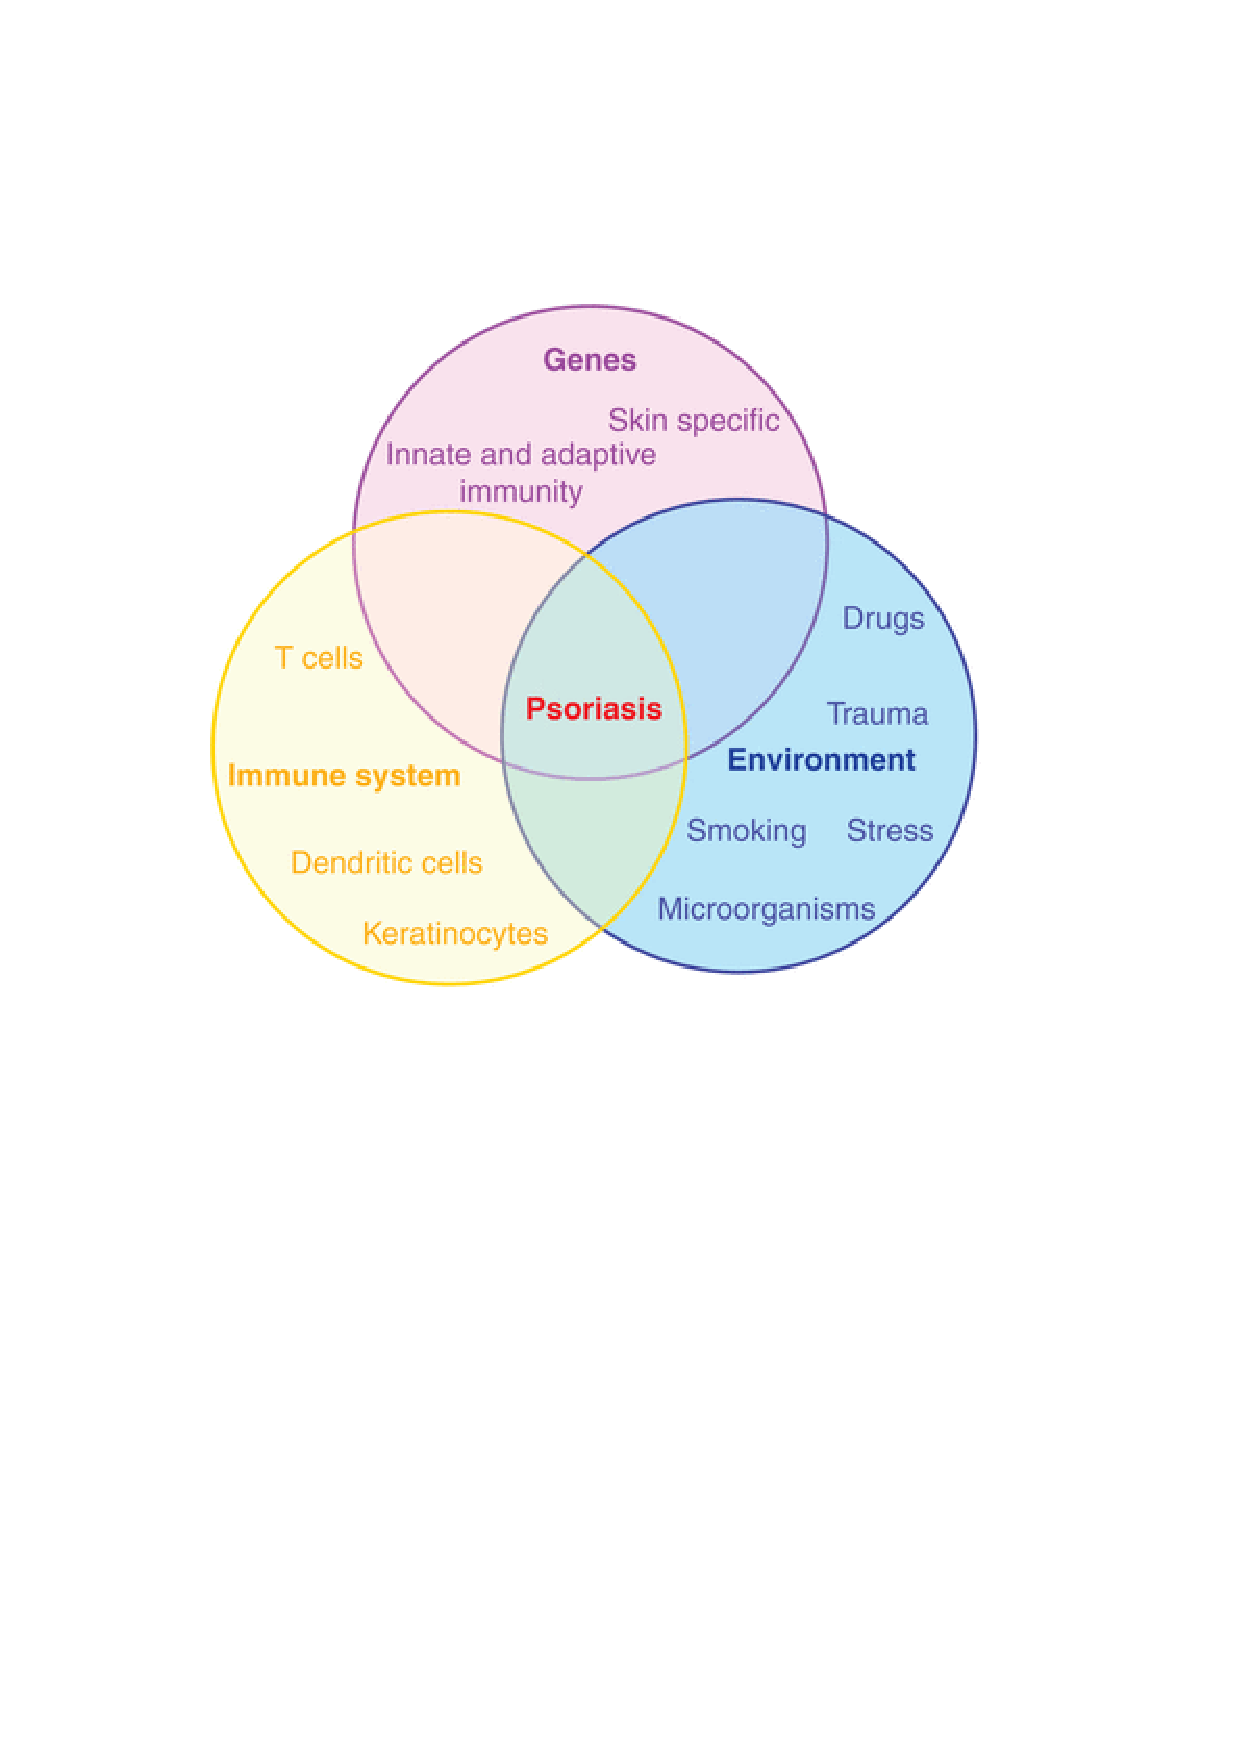
\includegraphics[width=\textwidth]{./Introduction/pdfs/PSO_aetiology_diagram_Di_Meglio_et_al_2014.pdf}
\caption[Main factors involved in PSO disease aetiology]{\textbf{Figure adapted from \parencite{Meglio2014}}}
\label{fig:PSO_aetiology_diagram}
\end{figure}

\textbf{HLA-C*06:02 mediated pathogenesis}
The association of the allele HLA-C*06:02 with PSO was first established through serological studies \parencite{Rusell1972, Tiilikainen1980} and it was later on confirmed the association of the region through genetic studies (Ellinghaus et al., 2010; Strange et al., 2010; Stuart et al., 2010; Sun et al., 2010)

the  identification of the precise gene within the associated region of the genome is challenging. Although some earlier studies using microsatellites as markers excluded HLA-C, later genetic studies using dense genotyping that allows better haplotype definition have confirmed HLA-C*06:02 as the susceptibility allele and have identified a single nucleotide polymorphism (SNP) within the gene to drive the greatest association  to disease \parencite{Nair2006, Nair2009} showing 10-fold increase of PSO risk in homozygosis \parencite{Perera2012}


number of HLA-C alleles 2375 encoding for 1677 proteins \parencite{Robinson2013}. Particularly, HLA-Cw*06 has 51 different subtypes 
Regarding allele frequency it changes among ethnic populations. 5553 British Caucasian individuals from the OBB HLA-C allele of greater frequency was HLA-C*07:01 (High resolution HLA haplotyping by imputation for a British population bioresource Neville2017)



Association of HLAC with other diseases such as Hepatitis C, PsA, primary sclerosing cholangitis and Grave´s disease \parencite{Blais2011}

However, the detailed role of HLA-C*06:02 in the pathogenesis of PSO remains uncertain partly due to the homology between different MHC-In and the polymorphic nature of HLA-C. 
	Presence of SNPs in minimal promoter and enhancer region that affects expression levels of HLA-C alleles \parencite{Clop2013, Hundhausen2012}. However HLA-Cw*0602 transcript levels do not differ significantly between normal and psoriatic showing responsiveness to proinflammatory cytokines and suggesting the association is not explained by alteration in regulation of gene expression \parencite{Hundhausen2012}. 
	Lack of functional studies showing specific antigen or interacting proteins recognised by this allele
	
HLA-C is  is a heterodimer consisting of a heavy chain and a light chain and expressed in the surface of most of the cells, including antigen presenting cells (APC); however it has lower expression levels and degree of polymorphism than HLA-A and HLA-B ( Low HLA-C expression at cell surfaces correlates with increased turnover of heavy chain mRNA).

 The major role of HLA-C has been assumed to be in acting as a ligand for killer immunoglobulin receptors (KIRs) expressed on natural killer (NK) cells however it is also recognised by TCR of CD8+ cells, not being clear if it exerts its pathogenic role through T cell or NK regulation 
APC can activate immune response through presentation of processed antigens to CD8+ T cells, very abundant in the lesional epidermis due to inflitration that antigen could be T cell recognition of self-peptides hypothesis reinforced by epistasia with ERAP1 \parencite{Strange2010}, which encodes for an aminopeptidase involved in the trimming of peptide antigens. ERAP1  locus  is  only  associated  with  PSO  in  individuals carrying the HLA-C risk allele. The presentation of autoantigens(Although there are some studies regarding the self-tolerance and presence of autoantigenes as disease trigger \parencite{Lande2007}, the autoimmune aetiology of PSO is still under debate) to CD8+ T cells that clonally expand in psoriasis lesions has been reinforced by the observation of melanocytes as skin-specific target cells of an HLA-C*06:02-restricted psoriatic T cell response. We found that a CD8+ TCR, which we had reconstituted from an epidermal CD8(+) T cell clone of an HLA-C*06:02-positive psoriasis patient specifically recognises HLA-C*06:02-positive melanocytes. we observed numerous CD8(+) T cells in psoriasis lesions attacking melanocytes, the only epidermal cells expressing ADAMTSL5. Furthermore, ADAMTSL5 stimulation induced the psoriasis signature cytokine, IL-17A %reinfoce 
, in CD8(+) T cells from psoriasis patients only, supporting a role as psoriatic autoantigen. % fact that CD4 are not reactive to autoantigen and that they are the first infiltrated cell type
This unbiased analysis of a TCR obtained directly from tissue-infiltrating CD8(+) T cells reveals that in psoriasis HLA-C*06:02 directs an autoimmune response against melanocytes through autoantigen presentation. We propose that HLA-C*06:02 may predispose to psoriasis via this newly identified autoimmune pathway \parencite{Arakawa2015}.

HLA-Cw*06:02 can be recognised by the inhibitory receptor KIR2DL1 and the activatory receptor KIR2DS1.  Some studies have shown KIR2DS1 was present in 85\% of the patients but only in 51\% of the controls
NK cells are important regulators of immune responses \parencite{Luszczek2004}. Their function extends beyond killing of infected or transformed cells. Interactions with dendritic cells, macrophages, and fetal trophoblast cells can regulate NK cell activity by influencing cytokine production, cytotoxicity and stimulation of T helper-1 responses. 


A similar inflammatory skin phenotype, which was also shown to be T-cell-dependent (Breban et al., 1996), was seen in rats transgenically expressing high levels of HLA-B27 and human β2-microglobulin (Tg(HLA-B*2705, B2M)33-3Trg; Table S1). However, these animals also developed multisystem inflammatory disease characterized by arthritis and colitis (Hammer et al., 1990).


\textbf{Histopathological alterations in skin and joints}

As previously mentioned, the epidermis is the most external structure of the skin and it is formed approximately by 90\% by keratinocytes (KC) organised in a layer structure that self-renews in a time dependent manner from the bottom to the surface \parencite{Wikramanayake2014}. As the KC differentiate they undergo changes in their ability to replicate, shape, keratin composition of the intracellular matrix and the formation of an cornified protein layer under the cell membrane. KC in the stratum corneum, the most superficial layer of the epidermis, are terminally differentiated, they lack of nuclei and they are surrounded by a cornified cell envelop consisting in protein rich and lipid rich layers \parencyte{Proskch2008, Wikramanayake2014}.

Alterations of the normal histological features of the epidermis due to dysregulation in the self-renewal process of this structure leads to development of the psoriatic lesions. Upregulation of the KC proliferation rate (hyperplasia) due to an acceleration in the turnover rate (from 28 to 8 days) causes aberrant cell differentiation characterised by incomplete cornification and presence of nuclei in the cells of the stratum corneum, phenomena known as parakeratosis. It also leads to thickening of the epidermis (acanthosis) and the subsequent scale formation. Concomitantly, inflammation causes immune cell infiltration and hypervascularisation of the lesion driven by upregulation in the expression of angiogenic factors such Vascular Endothelial Growth Factor (\textit{VEGF}) and activation of the endothelium \parencite{Perera2012}. As an example of the importance of this process in PSO development there is association with PSO risk of genes of the late cornified envelope (LCE) family within the epidermal cell differentiation complex \parencite{Tsoi2012}.

KC have been lately considered as immune sentinels with roles in antigen presentation and production of cytokines and chemokines that initiate and perpetuate the immune response. There is evidence of complex formed by the cationic antimicrobial peptide (AMP) LL-37 and fragments of self-DNA/RNA released by the damaged KC in the psoriatic skin \parencite{Lande2007}. Upon trigger of an environmental factor (section xxx) formation of this complex could lead to initiation of the skin inflammation through activation of skin-resident dendritic cells (DC) that release Interferon \gamma (IFN-\gamma) \parencite{Nestle2005}. Moreover, KC also secrete pro-inflammatory cytokines, importantly interleukin-1 (IL-1), which active form is processed by the inflammasome complex and reinforces activation of DC and Th lymphocytes \parencite{Feldmeyer2007, Arend2008}.%animal model of IL1??? 
Moreover, expression of the MHC-II allows KC to act as APC and activate memory CD4^+ and CD8^+ T cells inducing a recall immune response \parencite{Black2007}. KC also participate in the perpetuation of the inflammatory response in an independent manner, since they can be activated in absence of T cells upon xenobiotic stimuli \parencite{Griffiths1989} and they also produce inflammatory cytokines including IL-1, interleukin 6 (IL-6) and Tumor Necrotic Factor (TNF)-\alpha (TNF-\alpha), among others \parencite{Nestle2009}.

Following this relevant role of KC in the immune response, the ´outside-inside´ theory would attribute the chronic inflammatory response to the dysfunction of the  epidermis \parencyte{Proskch2008}. Some studies in animal models support this primary role of the epidermis in the initiation of disease. For example, mice without functional T cells still presented skin lesions; however they are weaker than the found in their counterpart wild type (ref). In addition to this, immunodeficient mice developed psoriatic lesions upon human xenotransplant of skin from PSO patients but not from healthy individuals \parencite{Boyman2004}. Overall, this reinforces the fact that underlying skin abnormality are partly responsible for driving the inflammatory.


\textbf{Dysregulation of the innate and adaptive immune response}
%link to the histological changes
Dysregulation of the immune response in PSO and PSA is the result of the interaction between innate and immune cells types (Section xx) as well as a complex cytokine milieu involving feedback loops.

As previously commented, KC play a very important role in the disease initiation (section xx). The proinflammatory cytokines produced by the activated KC induce the release of IFN-\alpha and IFN-\gamma by circulating plasmacytoid DC (pDC) and myeloid DC (mDC), respectively. They represent two of the most relevant cytokines in PSO and PsA pathogenesis and they contribute to lymphocyte recruitment and maintenance of DC activation (ref) and appear to be particularly upregulated at the mRNA level in the lesional skin \parencite{Schmid1994}. 

Another key cytokine in this dysregulated inflammatory process is TNF\alpha. It is produced by mast cells, Th1 and Th17 cells infiltrated in the psoriatic lesion and induces activation of Nuclear Factor kappa-light-chain-enhancer of activated B cells (NF-\kapaB) signaling pathways (ref). It also activates several kinase signaling pathways as well as cell death programs (ref). In the context of inflammation, NF-\kappaB represents a master transcriptional regulator of the innate and adaptive immune system that induces expression of proinflammatory cytokines, antiapoptotic genes and genes involved in chronic inflammation maintenance (ref). The importance of this transcription factor (TF) in PSO and PsA pathogenesis is reflected by the association with disease of several genetic variants in some of the negative regulators of its proinflammatory activity, including Nuclear Factor Of Kappa Light Polypeptide Gene Enhancer In B-Cells Inhibitor Alpha \textit{NFKBIA} and TNF Receptor-Associated Factor 3 Interacting protein 2 \textit{TRAF3IP2} (ref).
 
NF-\kappaB activation by \textit{TRAF3IP2} is also linked to IL-17 (https://www.ncbi.nlm.nih.gov/pmc/articles/PMC3580541/), a pivotal cytokine in a key loop for the maintenance of PSO and PsA inflammatory response, the interleukin-23 (IL-23) and Th17 axis. IL-23 is mainly produced by mDC and macrophages homing the inflamed skin and it binds to the IL-23 receptor (IL-23R), which expression is upregulated in the DC and T cells of the lesion and in circulating Th cells (ref). In PSO, IL-23 is the mediator for the pathogenic loop between activated KC and T cells (ref). Both IL-23 and IL-23R present protective and pathogenic genetic variants associated with PSO and PsA risk (ref). Activation of the IL-23 pathway leads importantly to increased IL-17 production that favors maintenance of the Th17 inflammatory response as well as KC activation (ref).

More recently, interleukin-22 (IL-22) has arisen as one of the key cytokines in mediating the dysregulated cross talk between the innate and adaptive immune response. IL-22 levels are increased in the psoriatic lesions and serum of patients and it is mainly produced by a subset of CD4^+ cells known as Th22 (ref). It mediates acanthosis and AMP production by KC (ref).


   




Nevertheless, other studies have demonstrated development of PSO in wild type mice upon bone marrow transplantation from mice with PSO-like phenotype







\textbf{Environmental factors and disease}
There are several environmental triggers known to be associated with increased risk and worsening of PSO and PsA development. A wide range of drugs including antidepressant, antihypertensive and anticytokine therapies have been clinically associated with initiation, exacerbation and worsening of PSO. As examples, therapies such as IFN-\alpha for the treatment of hepatitis C virus and anti-TNF antibodies for the treatment of several chronic inflammatory diseases, including PSO \parencite{Kim2010}.

Preceding streptococcal throat infection has likewise been associated with development of type I PSO lesions only \parencite{Gudjonsson2003}. This is partially explained by the molecular mimicry found for several streptococcal antigens, such as the M protein (highly similar to the structure of certain human keratins) and bacterial peptidoglycans \parencite{Valdimarsson2009}. Also, there is evidence of homologous T cell clones homing tonsils and psoriatic lesions \parencite{Diluvio2006}. Recent studies looking at the microbiome and disease development have suggested perturbation in the composition of the gut and skin microbiota of PSO and PsA patients compared to the controls \parencite{Yan2017}. Consistently with other chronic inflammatory disease such as IBD and AS, these differences in the microbiome could lead to dysregulation of inflammatory pathways in skin and joints through immunomodulation \parencite{Eppinga2014}.

Physical trauma, including tattoos and surgical incisions, has also been associated with the appearance of psoriatic lesions in uninvolved skin and joint inflammation in digits \parencite {Nestle2009} due to initiation of the Koebner phenomenon \parencite{Weiss2002}. Lastly, there are several behavioral factors such as smoking, alcohol and stress that have been suggested to be associated with PSO and PsA. However, there are not consistent conclusions of their involvement \parencite{Meglio2014}.




\subsection{Aetiology of PsA}


Identical T cell clonality between skin and synovium https://ac.els-cdn.com/S0198885999000348/1-s2.0-S0198885999000348-main.pdf?_tid=5efa7316-fde5-11e7-8091-00000aacb360&acdnat=1516454913_dd20efb867f822d68d8b09873601e8ad

Process that leads to disease. Maybe I can talk about the skin and how it leads to the lesions,summary of how disease occurs and about autoimmunity. Same for PsA
Include environmental risk factors







%
\subsection*{Cell types involved in pathophysiology}
%Global report on psoriasis, 2016

\subsection*{Therapeutic intervention}
%


\subsection*{GWAS and functional genomics of psoriasis and other complex diseases}
\subsubsection*{Epigenetics and gene expression}
\textbf{Understanding the chromatin landscape}
\textbf{Chromatin accessibility}
\textbf{Histones modifications}
\textbf{Understanding the chromatin landscape}
\textbf{Transcription factor occupancy}
\textbf{Chromatin interaction}

\begin{figure}[H]
\includegraphics[width=\textwidth]{./Introduction/eQTL.pdf}%
\caption[Effect of regulatory variants on expression levels of genes]{\textbf{Effect of regulatory variants on expression levels of genes}. Reprinted by permission from Macmillan Publishers Ltd: Nature Reviews Genetics \parencite{Cheung2009}, copyright 2009. The effect of local (\textit{cis}) or distal (\textit{trans}) regulatory variants on levels of gene expression.}%
\label{fig:intro.eQTL}%
\end{figure}


\section{Sepsis}
Sepsis is defined as the systemic inflammatory response to the presence of an infection and is classified as severe when associated with organ dysfunction, hypoperfusion abnormality or sepsis-induced hypotension.  Systemic inflammatory response syndrome (SIRS) is used to describe the inflammatory response and it includes at least two of the clinical manifestations detailed in Table \ref{tab:SIRS.sepsis} \parencite{Bone1992}.  However this definition is limited in that the microbiological basis of the response is not considered and there is no graduation of severity.  In the UK, severe sepsis accounts for 27\% of ICU admissions \parencite{Padkin2003} and from a number of studies in both the UK and America, mortality has been estimated to be between 28\% and 50\% \parencite{Angus2001, Padkin2003, Sands1997, Zeni1997}. \\
%\ToDo{Table 1.2 in Jay't thesis, revised criteria in 2001?}.

\begin{table}[H]
\centering\doublespacing
\caption[The clinical manifestations of SIRS]{\textbf{The clinical manifestations of SIRS \parencite{Bone1992}.} SIRS is diagnosed in patients with at least two of these clinical manifestations.}  
\label{tab:SIRS.sepsis}
\begin{tabular}{>{\centering\arraybackslash}m{0.9\textwidth}}
\\ \toprule
\textbf{SIRS clinical manifestations} \\ 
\midrule
Body temperature \textgreater 38\degree C \\
Heart rate \textgreater 90 beats per minute \\
Respiratory rate \textgreater 20 breaths per minute or hyperventilation \newline as indicated by a PACO\textsubscript{2} of \textless 32 mm Hg \\
An alteration in the white blood cell count (count \textgreater 12,000/cu mm or \newline \textless 400/cu mm or the presence of \textgreater 10\% immature neutrophils)\\
\bottomrule
\end{tabular}
\end{table}



%%%%%%%%%%%%%%%%%%%%%%%%%%%%%%%
\section{Common variable immune deficiency disorders}

Primary immunodeficiencies (PIDs) are a group of rare disorders that result from a failure in the immune system and CVID are the most frequently encountered PID in the clinic \parencite{Park2008}. CVID are a group of diseases in which insufficient quantity and quality of immunoglobulin usually leads to susceptibility to recurrent bacterial infections, mainly of the respiratory and gastrointestinal tracts \parencite{Chapel2009}.  An immunodeficiency is recognized in most CVID patients in the second, third or fourth decade of life and the first diagnostic criteria were published in 1999 (Table~\ref{tab:criteria.cvid}) \parencite{Conley1999}.  These criteria have been used since then with slight variations for example, the minimum age of presentation is often increased to 4 years in order to avoid infants with immune defects which cause B cell differentiation and class-switch disorders \parencite{Chapel2008}.

\begin{table}[H]
\centering
\singlespacing
\caption[CVID diagnosis criteria]{\textbf{CVID diagnosis criteria.} Individuals fulfilling each of the criteria are diagnosed with CVID \parencite{Conley1999}. SD = standard deviations.}  
\label{tab:criteria.cvid}
\begin{tabular}{c}
\toprule
\textbf{Criteria for CVID diagnosis} \\ 
\midrule
Male or female patient \textgreater 2 years of age\\
Serum IgG and IgA at least 2 SD below the mean for age \\
IgM is present or absent\\
Poor response to vaccines \\
Absent isohemagglutinins \\
Defined causes of hypogammaglobulinemia have been excluded \\
Normal or low B cell numbers \\
\bottomrule
\end{tabular}
\end{table} 

%%%
\subsection{Clinical complications}
The diagnosis of CVID is made by excluding known disorders of B cell failure for example B cell differentiation defects resulting in absent B cells, activation-induced cytidine deaminase (AID) and uracil-DNA glycosylase (UNG) deficiencies affecting B cell function and T cell switching pathways \parencite{Chapel2008}. This results in a heterogeneous group of individuals with widely different clinical features and additional complications.

Within cohorts of CVID patients, beyond bacterial infections, the main clinical complications observed include autoimmunity, lymphocytic infiltration, enteropathy and malignancy (Figure~\ref{fig:complications.intro.cvid}). Patients with at least one clinical complication have a much poorer survival rate compared to those with an Infections Only phenotype \parencite{Chapel2008}.

\begin{figure}[H]
\centering
\begin{subfigure}[b]{0.49\textwidth}
	\centering
	\includegraphics[width=\textwidth]{./Introduction/Barplot_complications_cvid.pdf}%
	\caption{Number of complications}%
\end{subfigure}
\begin{subfigure}[b]{0.49\textwidth}
	\centering
	\includegraphics[width=\textwidth]{./Introduction/Pie_1complication.pdf}%
	\caption{One complication}%
\end{subfigure}
\begin{subfigure}[b]{0.49\textwidth}
	\centering
	\includegraphics[width=\textwidth]{./Introduction/Pie_2complication.pdf}%
	\caption{Two complications}%
\end{subfigure}
\begin{subfigure}[b]{0.49\textwidth}
	\centering
	\includegraphics[width=\textwidth]{./Introduction/Pie_3complication.pdf}%
	\caption{Three complications}%
\end{subfigure}
\caption[Nature and number of CVID complications]{\textbf{Nature and number of CVID complications.} a) Number of complications observed in each individual. Individuals with no complications are referred to as infections only. b) Distribution of complications in patients with one complication. c)  Distribution of complications in patients with two complications. d)  Distribution of complications in patients with three complications. \parencite{Chapel2008}}
\label{fig:complications.intro.cvid}
\end{figure}


